%!TEX root = ../main.tex

\section{Approach}
\label{sec:mathematical_formulation}

The minimum time optimal control problem can be generically formulated as follows:

\textbf{Cost}: $$J=\int_{t_{0}}^{t_{f}} d t$$

\textbf{Nonlinear Dynamics:} $$\dot{x}(t)= f(x(t), u(t), t)$$

\textbf{Constraints:} 
\begin{itemize}
  \item Input constraints:
    $$M_{i}^{-} \leq u_{i}(t) \leq M_{i}^{+}$$
  \item Path constraints:
  $\forall t, t_{0} \leq t \leq t_{f}$ 
  $$c(x(t), u(t), t) \leq 0,$$
\end{itemize}

\textbf{Boundary Conditions:}
Given 
\begin{itemize}
  \item Initial: $n(x(t_{0}), t_{0}) = 0$
  \item Final: $m(x(t_{f}), t_{f}) = 0$
\end{itemize}

\subsection{Mathematical Model of a Quadcopter}

Absolute position: $x, y, z$.

Attitude: pitch $\theta$, roll $\phi$, yaw $\psi$.

$$\boldsymbol{\xi}=\left[ \begin{array}{l}{x} \\ {y} \\ {z}\end{array}\right], \quad \boldsymbol{\eta}=\left[ \begin{array}{l}{\phi} \\ {\theta} \\ {\psi}\end{array}\right]$$

Linear velocities (body frame): $\boldsymbol{V}_{B}$

Angular velocities (body frame): $\boldsymbol{\nu}$

$$\boldsymbol{V}_{B}=\left[ \begin{array}{c}{v_{x, B}} \\ {v_{y, B}} \\ {v_{z, B}}\end{array}\right], \quad \boldsymbol{\nu}=\left[ \begin{array}{l}{p} \\ {q} \\ {r}\end{array}\right]$$

The rotation matrix from the body frame ($B$) to the inertial frame ($G$) is given by:
$\mathbf{x}^{B}=\mathbf{R}_{G}^{B} \mathbf{X}^{G}=\mathbf{R}(\phi) \mathbf{R}(\theta) \mathbf{R}(\psi) \mathbf{X}^{G}$

$$\boldsymbol{R}_B^G=\boldsymbol{R}=\left[ \begin{array}{ccc}{C_{\psi} C_{\theta}} & {C_{\psi} S_{\theta} S_{\phi}-S_{\psi} C_{\phi}} & {C_{\psi} S_{\theta} C_{\phi}+S_{\psi} S_{\phi}} \\ {S_{\psi} C_{\theta}} & {S_{\psi} S_{\theta} S_{\phi}+C_{\psi} C_{\phi}} & {S_{\psi} S_{\theta} C_{\phi}-C_{\psi} S_{\phi}} \\ {-S_{\theta}} & {C_{\theta} S_{\phi}} & {C_{\theta} C_{\phi}}\end{array}\right]$$

where $S_{x}=\sin (x)$ and $C_{x}=\cos (x)$.

Time derivative of this rotation matrix provides us with the angular velocities. These are not simply the time derivatives of the independent Euler angles, instead:

$\dot{\boldsymbol{\eta}}=\boldsymbol{W}_{\eta}^{-1} \boldsymbol{\nu}$, \hfill $\left[ \begin{array}{c}{\dot{\phi}} \\ {\dot{\theta}} \\ {\dot{\psi}}\end{array}\right]=\left[ \begin{array}{ccc}{1} & {S_{\phi} T_{\theta}} & {C_{\phi} T_{\theta}} \\ {0} & {C_{\phi}} & {-S_{\phi}} \\ {0} & {S_{\phi} / C_{\theta}} & {C_{\phi} / C_{\theta}}\end{array}\right] \left[ \begin{array}{l}{p} \\ {q} \\ {r}\end{array}\right]$

Conversely,

$\boldsymbol{\nu}=\boldsymbol{W}_{\eta} \dot{\boldsymbol{\eta}}, \hfill \left[ \begin{array}{l}{p} \\ {q} \\ {r}\end{array}\right]=\left[ \begin{array}{ccc}{1} & {0} & {-S_{\theta}} \\ {0} & {C_{\phi}} & {C_{\theta} S_{\phi}} \\ {0} & {-S_{\phi}} & {C_{\theta} C_{\phi}}\end{array}\right] \left[ \begin{array}{c}{\dot{\phi}} \\ {\dot{\theta}} \\ {\dot{\psi}}\end{array}\right]$
  
where $T_{x}=\tan (x)$.
The matrix $\boldsymbol{W}_{\eta}$ is invertible if $\theta \neq(2 k-1) \phi / 2,(k \in \mathbb{Z})$

\begin{table}[htbp]
  \begin{tabular}{|c|p{0.8\linewidth}|}
    \hline \text{Symbol} & \text{Definition} \\
    \hline 
    {$\boldsymbol{\xi}$} & {Absolute position (inertial frame)} \\
    {$\boldsymbol{\eta}$} & {Attitude (inertial frame)} \\
    {$\boldsymbol{V}_B$} & {Linear velocities (body frame)} \\
    {$\boldsymbol{\nu}$} & {Angular velocities (body frame)} \\
    {$\boldsymbol{\mathrm{R}}$} & {Rotation matrix from body to inertial frame} \\
    {$\boldsymbol{\mathrm{W}_\eta}$} & {Transformation matrix for angular velocities from inertial to body frame} \\
    {$\boldsymbol{I}$} & {Inertia matrix} \\
    {$\boldsymbol{G}$} & {Gravity} \\
    \hline
  \end{tabular}
  \caption{Definitions and Notations}
\end{table}

\textbf{Assumptions}:
\begin{itemize}
  \item The quadrotor structure is rigid and symmetrical with a center of mass aligned with the
  center of the body frame of the vehicle. The four arms of the quadcopter are aligned with the body x- and y-axes.
  Therefore, the inertia matrix $\textbf{I}$ is diagonal:

  $$\boldsymbol{I}=\left[ \begin{array}{ccc}{I_{x x}} & {0} & {0} \\ {0} & {I_{y y}} & {0} \\ {0} & {0} & {I_{z z}}\end{array}\right]$$

    We further have that due to symmetry inertial components are equal: $I_{xx}=I_{yy}$.

  \item The thrust and drag of each motor is proportional to the square of the motor velocity.
  \item The propellers are considered to be rigid and therefore blade flapping is negligible
    (deformation of propeller blades due to high velocities and flexible material. 
  \item The Earth is flat and non-rotating (difference of gravity by altitude or the spin of the earth
  is negligible)
  \item Surrounding fluid velocities (wind) are negligible. 
  \item Ground effect is negligible.
\end{itemize}

These assumptions and basic dynamics lead to the model used in this work.
The following derivations are a summary of the equations in \cite{}.

\begin{figure}[htbp]
  \centering
  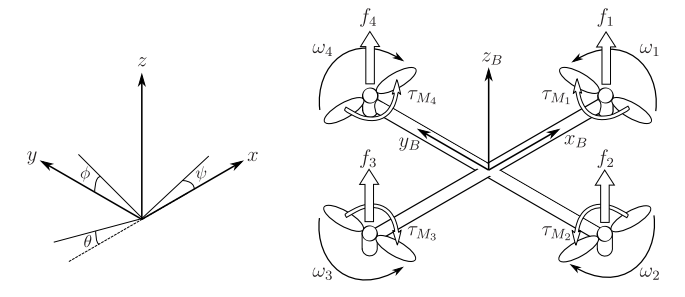
\includegraphics[width=\linewidth]{img/reference_frames.png}
  \caption{The inertial and body frames of a quadcopter (ENU coordinates). Figure from \cite{TODO}.}
  \label{fig:reference_frames}
\end{figure}

\subsection{Quadcopter Dynamics}
\begin{itemize}
  \item The angular velocity of rotor $i,$ denoted with $\omega_{i},$ creates force $f_{i}$ in the direction of
the rotor axis: 
$$f_{i}=k \omega_{i}^{2}$$

The combined forces of rotors create thrust $T$ in the direction of the body z-axis.

$$T=\sum_{i=1}^{4} f_{i}=k \sum_{i=1}^{4} \omega_{i}^{2}, \quad \quad \boldsymbol{T}_{B}=\left[ \begin{array}{c}{0} \\ {0} \\ {T}\end{array}\right]$$

  \item The angular velocity and acceleration of the rotor also creates torque $\tau_{M_i}$ around the rotor axis: 
  $$I_{M} \dot{\omega}_{i} = \tau_{M_{i}} - b \omega_{i}^{2}$$
  in which the lift constant is $k,$ the drag constant is $b$ and the inertia moment of the
rotor is $I_{M}$. 

Usually the acceleration of the rotor ($\dot{\omega}_{i}$) is considered small and thus it is omitted.
  This holds when we assume that the quadrotor is operating in stable flight and that the propellers are maintaining a constant thrust and not accelerating.
  This assumption results in the torque about the global z axis being equal to the torque due to drag.

Torque $\boldsymbol{\tau_B}$ consists of the torques on the three axis $\tau_\phi, \tau_\theta, \tau_\psi$:

$$
\boldsymbol{\tau}_{B}=\left[ \begin{array}{c}{\tau_{\phi}} \\ {\tau_{\theta}} \\ {\tau_{\psi}}\end{array}\right]=
\left[ \begin{array}{c}{l k\left(-\omega_{2}^{2}+\omega_{4}^{2}\right)} \\ {l k\left(-\omega_{1}^{2}+\omega_{3}^{2}\right)} \\ {\sum_{i=1}^{4} (-1)^{i+1} \tau_{M_{i}}}\end{array}\right]
  $$
  $$
  =
\left[ \begin{array}{c}
{l k\left(-\omega_{2}^{2}+\omega_{4}^{2}\right)} \\
{l k\left(-\omega_{1}^{2}+\omega_{3}^{2}\right)} \\
{b(\omega_{1}^{2}-\omega_{2}^{2}+\omega_{3}^{2}-\omega_{4}^{2})}\end{array}\right]
  $$

where $l$ is the distance between the rotor and the center of mass of the quadcopter.

\end{itemize}


\subsubsection{Translational dynamics}

Newton's second law: 
$$m \ddot{\boldsymbol{\xi}}=\boldsymbol{G}+\boldsymbol{R} \boldsymbol{T}_{B}$$

$$\left[ \begin{array}{c}{\ddot{x}} \\ {\ddot{y}} \\ {\ddot{z}}\end{array}\right]=-g \left[ \begin{array}{l}{0} \\ {0} \\ {1}\end{array}\right]+\frac{T}{m} \left[ \begin{array}{c}{C_{\psi} S_{\theta} C_{\phi}+S_{\psi} S_{\phi}} \\ {S_{\psi} S_{\theta} C_{\phi}-C_{\psi} S_{\phi}} \\ {C_{\theta} C_{\phi}}\end{array}\right]$$

\subsubsection{Rotational dynamics}
The rotational equations of motion are defined in the body frame so that the rotations can be computed about the quadrotor’s center and not the center of the global coordinate frame.

Applying Euler's second law:
$$\boldsymbol{I} \dot{\nu}+\boldsymbol{\nu} \times(\boldsymbol{I} \boldsymbol{\nu})+\mathbf{\Gamma}=\boldsymbol{\tau}$$
where:
\begin{itemize}
  \item Angular acceleration of the inertia: $\boldsymbol{I\dot{v}}$
  \item Centripetal forces: $\boldsymbol{\nu}\times(\boldsymbol{I \nu})$
  \item Gyroscopic forces: $\boldsymbol{\Gamma}$
  \item External torque: $\boldsymbol{\tau}_B$
\end{itemize}

Replacing terms by their definitions, multiplying both sides by $\boldsymbol{I}^{-1}$, and rearranging:
$$\boldsymbol{\dot{\nu}}=\boldsymbol{I}^{-1}\left(-\left[ \begin{array}{c}{p} \\ {q} \\ {r}\end{array}\right] \times \left[ \begin{array}{c}{I_{x x} p} \\ {I_{y y} q} \\ {I_{z z} r}\end{array}\right]-I_{r} \left[ \begin{array}{c}{p} \\ {q} \\ {r}\end{array}\right] \times \left[ \begin{array}{c}{0} \\ {0} \\ {1}\end{array}\right] \omega_{\Gamma}+\boldsymbol{\tau}_B\right)$$

$$
\begin{array}{c}
\left[ \begin{array}{c}{\dot{p}} \\ {\dot{q}} \\ {\dot{r}}\end{array}\right]= 
\left[ \begin{array}{c}{\left(I_{y y}-I_{z z}\right) q r / I_{x x}} \\ {\left(I_{z z}-I_{x x}\right) p r / I_{y y}} \\ {(I_{x x}-I_{y y}) p q / I_{z z}}\end{array}\right] 
- I_{r} \left[ \begin{array}{c}{q / I_{x x}} \\ {-p / I_{y y}} \\ {0}\end{array}\right] \omega_{\Gamma} \\
+ \left[ \begin{array}{c}{\tau_{\phi} / I_{x x}} \\ {\tau_{\theta} / I_{y y}} \\ {\tau_{\psi} / I_{z z}}\end{array}\right]
\end{array}
  $$

  where $\omega_\Gamma = \omega_1 - \omega_2 + \omega_3 - \omega_4$, and $I_r$ is the rotor moment of inertia.


The angular accelerations in world frame $\ddot{\boldsymbol{\eta}}$ are given by the time derivatives of the angular velocities $\left(\dot{\boldsymbol{\eta}} = \boldsymbol{W}_{\eta}^{-1} \boldsymbol{\nu}\right)$,

$$\ddot{\boldsymbol{\eta}}=\frac{\mathrm{d}}{\mathrm{d} t}\left(\boldsymbol{W}_{\eta}^{-1} \boldsymbol{\nu}\right) =\frac{\mathrm{d}}{\mathrm{d} t}\left(\boldsymbol{W}_{\eta}^{-1}\right) \boldsymbol{\nu}+\boldsymbol{W}_{\eta}^{-1} \dot{\boldsymbol{\nu}} = $$

$$
\begin{array}{c}
\left[ \begin{array}{cccc}{0} & {\dot{\phi} C_{\phi} T_{\theta}+\dot{\theta} S_{\phi} / C_{\theta}^{2}} & {-\dot{\phi} S_{\phi} C_{\theta}+\dot{\theta} C_{\phi} / C_{\theta}^{2}} \\ {0} & {-\dot{\phi} S_{\phi}} & {-\dot{\phi} C_{\phi}} \\ {0} & {\dot{\phi} C_{\phi} / C_{\theta}+\dot{\phi} S_{\phi} T_{\theta} / C_{\theta}} & {-\dot{\phi} S_{\phi} / C_{\theta}+\dot{\theta} C_{\phi} T_{\theta} / C_{\theta}}\end{array}\right] \boldsymbol{\nu}
\\ + \boldsymbol{W_{\eta}^{-1}} \dot{\boldsymbol{\nu}}.
\end{array}
  $$

At this point, it is common to do a simplification by setting $[\dot{\phi} \quad \dot{\theta} \quad \dot{\psi}]^{T}=\left[ \begin{array}{lll}{p} & {q} & {r}\end{array}\right]^{T}$, which holds true for small angles of movement \cite{Sabatino}.
  \TODO{The equations below were taken from Will Selby's paper and they are apparently with typos, $\ddot{y}$'s $\sin(\psi)$ should be $\cos(\psi)$}

$\begin{aligned} 
 \ddot{x} &=\frac{(\cos \phi \sin \theta \cos \psi+\sin \phi \sin \psi) u_{1}-K_{f x} \dot{x}}{m} \\
 \ddot{y} &=\frac{(\sin \phi \sin \theta \cos \psi-\sin \phi \cos \psi) u_{1}-K_{f y} \dot{x}}{m} \\
 \ddot{z} &=\frac{(\cos \phi \cos \theta) u_{1}-K_{f z} \dot{z}}{m}-g 
\end{aligned}$
$\begin{aligned} \ddot{\phi} &=\frac{l\left(u_{2}-K_{l} \dot{\phi}\right)}{I_{x}} \\ \ddot{\theta} &=\frac{l\left(u_{3}-K_{l} \dot{\theta}\right)}{I_{y}} \\ \ddot{\psi} &=\frac{\left(u_{4}-K_{d} \dot{\psi}\right)}{I_{z}} \end{aligned}$

\subsection{Aerodynamic Drag}

\begin{itemize}

  \item We include the drag force generated by the air resistance. For this, we add a diagonal coefficient matrix that associates the linear velocities to the force slowing the movement

  $$
    \begin{array}{l}
      \left[ \begin{array}{l}{\ddot{x}} \\ {\ddot{y}} \\ {\ddot{z}}\end{array}\right]=-g \left[ \begin{array}{l}{0} \\ {0} \\ {1}\end{array}\right]+\frac{T}{m} \left[ \begin{array}{c}{C_{\psi} S_{\theta} C_{\phi}+S_{\psi} S_{\phi}} \\ {S_{\psi} S_{\theta} C_{\phi}-C_{\psi} S_{\phi}} \\ {C_{\theta} C_{\phi}}\end{array}\right] \\
      - \frac{1}{m} \left[ \begin{array}{ccc}{A_{x}} & {0} & {0} \\ {0} & {A_{y}} & {0} \\ {0} & {0} & {A_{z}}\end{array}\right] \left[ \begin{array}{c}{\dot{x}} \\ {\dot{y}} \\ {\dot{z}}\end{array}\right]
    \end{array}
  $$

  in which $A_{x}, A_{y}$ and $A_{z}$ are the drag force coefficients for velocities in the corresponding directions of the inertial frame.

  Several other aerodynamical effects could be included in the model. For example,
dependence of thrust on angle of attack, blade flapping and airflow disruptions.

  \item We ignore rotational drag forces since we assume rotational velocities to be relatively low. Alternatively,
   we could add the components $\boldsymbol{\tau}_{\boldsymbol{w}}=\left[ \begin{array}{lll}{\tau_{w x}} & {\tau_{w y}} & {\tau_{w z}}\end{array}\right]^{T}$ to the overall torque.

\end{itemize}

\subsection{State-space Model}

We can write our nonlinear dynamics using the following state vector:

$\boldsymbol{X}^{T}=\left[\begin{array}{cccccccccccc}{x} & {y} & {z} & {\dot{x}} & {\dot{y}} & {\dot{z}} & {\phi} & {\theta} & {\psi} & {p} & {q} & {r}\end{array}\right]^{T}$

Moreover, we define our inputs as follow:
\begin{itemize}
  \item $U_1$: the resulting thrust of the four rotors.
  \item $U_2$: the difference of thrust between the motors on the $x$ axis which results in roll angle changes and subsequent movement in the lateral x direction.
  \item $U_3$: the difference of thrust between the motors on the y axis which results in pitch
  angle changes and subsequent movement in the lateraly direction.
  \item $U_4$: the difference of torque between the clockwise and counterclockwise rotors which
  results in a moment that rotates the quadrotor around the vertical z axis.
\end{itemize}

$$U=\left[ \begin{array}{l}{U_{1}} \\ {U_{2}} \\ {U_{3}} \\ {U_{4}}\end{array}\right]= \left[ \begin{array}{c}{T} \\ {\tau_{\phi}} \\ {\tau_{\theta}} \\ {\tau_{\psi}}\end{array}\right]=
\left[ \begin{array}{c}
{k \sum_{i=1}^{4} \omega_{i}^{2}} \\
{l k\left(-\omega_{2}^{2}+\omega_{4}^{2}\right)} \\ 
{l k\left(-\omega_{1}^{2}+\omega_{3}^{2}\right)} \\ 
{b(\omega_{1}^{2}-\omega_{2}^{2}+\omega_{3}^{2}-\omega_{4}^{2})}\end{array}\right]
$$

Our nonlinear dynamics can be written as a nonlinear differential equation of the states $\boldsymbol{X}$ and control inputs $\boldsymbol{U}$:
$\dot{\boldsymbol{X}}=f(\boldsymbol{X}, \boldsymbol{U}).$

Or, more precisely:
$$
\dot{\boldsymbol{X}} = 
\left[
\begin{array}{c}
\dot{x} \\
{}\\
\dot{y} \\
{}\\
\dot{z} \\
{}\\
{}\\
\ddot{x} \\
{}\\
\ddot{y} \\
{}\\
\ddot{z} \\
{}\\
{}\\
\dot{\phi} \\
{}\\
\dot{\theta} \\
{}\\
\dot{\psi} \\
{}\\
{}\\
\dot{p} \\
{}\\
\dot{q} \\
{}\\
\dot{r}
\end{array}
\right]
=
\left[
\begin{array}{l}

\dot{x} \\
{}\\
\dot{y} \\
{}\\
\dot{z} \\
{}\\
{}\\
  -\frac{T}{m}[S_{\phi} S_{\psi}+C_{\phi} C_{\psi} S_{\theta}] \\
{}\\
  -\frac{T}{m}[C_{\phi} S_{\psi} S_{\theta}-C_{\psi} S_{\phi}] \\
{}\\
  g-\frac{T}{m}[C_{\phi} C_{\theta}] \\
  \TODO{\text{Li estem ficant drag nosaltres}}
{}\\
{}\\
  p+r[C_{\phi} T_{\theta}]+q[S_{\phi} T_{\theta}] \\
{}\\
  q[C_{\phi}]-r[S_{\phi}] \\
{}\\
  r \frac{C_{\phi}}{C_{\theta}}+q \frac{S_{\phi}}{C_{\theta}} \\
{}\\
{}\\
\frac{I_{y}-I_{z}}{I_{x}} r q - \frac{I_r}{I_{x}} q w_{\Gamma} +\frac{\tau_{\phi}}{I_{x}} \\
{}\\
\frac{I_{z}-I_{x}}{I_{y}} p r + \frac{I_r}{I_{y}} p w_{\Gamma} +\frac{\tau_{\theta}}{I_{y}} \\
{}\\
\frac{I_{x}-I_{y}}{I_{z}} p q +\frac{\tau_{\psi}}{I_{z}}
\end{array}
\right]
=f(\boldsymbol{X}, \boldsymbol{U})
$$


\subsection{Simplifications}
\label{ssec:frontend}

The primary assumption made to simplify the model is that the quadrotor will be operated around a stable hover with small attitude angles and minimal rotational and translational velocities and accelerations.
Since there are no aerodynamic lifting surfaces, we will assume that the aerodynamic forces and moments are negligible.
The effects that are considered negligible are treated as disturbances in the control system and can be compensated for with appropriate control system design.
These assumptions are described mathematically as well as the resulting simplified equations of motion.
The equations below continue to reduce in complexity as more assumptions are made.

$
\left\{
\begin{array}{l}
  f_{t}=b\left(\Omega_{1}^{2}+\Omega_{2}^{2}+\Omega_{3}^{2}+\Omega_{4}^{2}\right) \\
  \tau_{x}=b l\left(\Omega_{3}^{2}-\Omega_{1}^{2}\right) \\
  \tau_{y}=b l\left(\Omega_{4}^{2}-\Omega_{2}^{2}\right) \\
  \tau_{z}=d\left(\Omega_{2}^{2}+\Omega_{4}^{2}-\Omega_{1}^{2}-\Omega_{3}^{2}\right)
\end{array}
\right.
$

Define control inputs as:

$$U=\left[ \begin{array}{l}{U_{1}} \\ {U_{2}} \\ {U_{3}} \\ {U_{4}}\end{array}\right]=\left[ \begin{array}{c}{T_{1}+T_{2}+T_{3}+T_{4}} \\ {T_{4}-T_{2}} \\ {T_{3}-T_{1}} \\ {\left(T_{1}+T_{3}\right)-\left(T_{2}+T_{4}\right)}\end{array}\right]$$
where $T_i=b\omega_{i}^2$ is the thrust force of propeller $i$.

  Using the following constants for simplifying the equations:
$$a_{1}=\frac{I_{y y}-I_{z z}}{I_{x x}}, \quad a_{2}=\frac{I_{z z}-I_{x x}}{I_{y y}}, \quad a_{3}=\frac{I_{x x}-I_{y y}}{I_{z z}}$$

$$b_{1}=\frac{l}{I_{x x}}, \quad b_{2}=\frac{l}{I_{y y}}, \quad b_{3}=\frac{l}{I_{z z}}$$

We get:

$$
\left[ \begin{array}{l}
\ddot{\phi} \\ \ddot{\theta} \\ \ddot{\psi} 
\end{array} \right] = 
\left[ \begin{array}{l}
\frac{I_{yy}-I_{zz}}{I_{xx}} \dot{\theta} \dot{\psi} + \frac{\tau_{x}}{I_{xx}} \\ 
\frac{I_{zz}-I_{xx}}{I_{yy}} \dot{\phi} \dot{\psi} + \frac{\tau_{y}}{I_{yy}} \\
\frac{I_{xx}-I_{yy}}{I_{zz}} \dot{\phi} \dot{\theta} + \frac{\tau_{z}}{I_{zz}} 
\end{array}\right]
=
\left[ \begin{array}{l}
a_1 \dot{\theta} \dot{\psi} + b_1 u_2 \\ 
a_2 \dot{\phi} \dot{\psi} + b_2 u_3 \\
a_3 \dot{\phi} \dot{\theta} + b_3 u_4
\end{array}\right]
$$

Using these together with the absolute acceleration above:

$$\left[ \begin{array}{c}{\ddot{x}} \\ {\ddot{y}} \\ {\ddot{z}}\end{array}\right]=-g \left[ \begin{array}{l}{0} \\ {0} \\ {1}\end{array}\right]+\frac{T}{m} \left[ \begin{array}{c}{C_{\psi} S_{\theta} C_{\phi}+S_{\psi} S_{\phi}} \\ {S_{\psi} S_{\theta} C_{\phi}-C_{\psi} S_{\phi}} \\ {C_{\theta} C_{\phi}}\end{array}\right]$$

\subsubsection{Calculus of Variations}
\label{sssec:3d_mesh_generation}

\subsubsection{3D Mesh Propagation}
